% Figure 1 -- PCF-SPR sensor cross-section, redrawn in TikZ for the SIVP submission.
%
% The conference paper used a raster screenshot exported from the COMSOL model
% (Figx.png): a split disc with the coloured geometry on the left half and the
% FEM mesh on the right half, green PML ring, blue analyte channel, brown silica
% core region, and r1/r2/r3/rc arrow annotations.
%
% This version is an independent vector drawing of the same published design:
%   * full geometry, not a split disc; the mesh half is dropped
%   * new palette (slate silica, pale-blue analyte, gold ring, grey PML)
%   * air holes drawn as unfilled circles with a hairline rule, not white discs
%   * the three cladding-hole families are keyed by hatch/edge weight and a
%     legend, instead of in-figure arrows to each radius
%   * pitch shown as a lattice vector between two adjacent hole centres
%   * all callouts re-lettered to the symbols used in the manuscript text
%
% Build standalone:
%   pdflatex fig1_cross_section.tex && mv fig1_cross_section.pdf ../figs/
% Or \input this body into the manuscript inside a tikzpicture-capable float.

\documentclass[border=2pt,tikz]{standalone}
\usepackage{amsmath}
\usetikzlibrary{calc,patterns,arrows.meta,positioning}

% --- palette (deliberately unlike the conference raster) ---------------------
\definecolor{silica}{HTML}{E8E6F0}
\definecolor{analyte}{HTML}{D6EAF6}
\definecolor{goldlayer}{HTML}{EDA100}
\definecolor{pml}{HTML}{EFEFEF}
\definecolor{holeedge}{HTML}{4A3AA7}
\definecolor{ink}{HTML}{1A1A1A}
\definecolor{inkmuted}{HTML}{6B6B6B}

\begin{document}
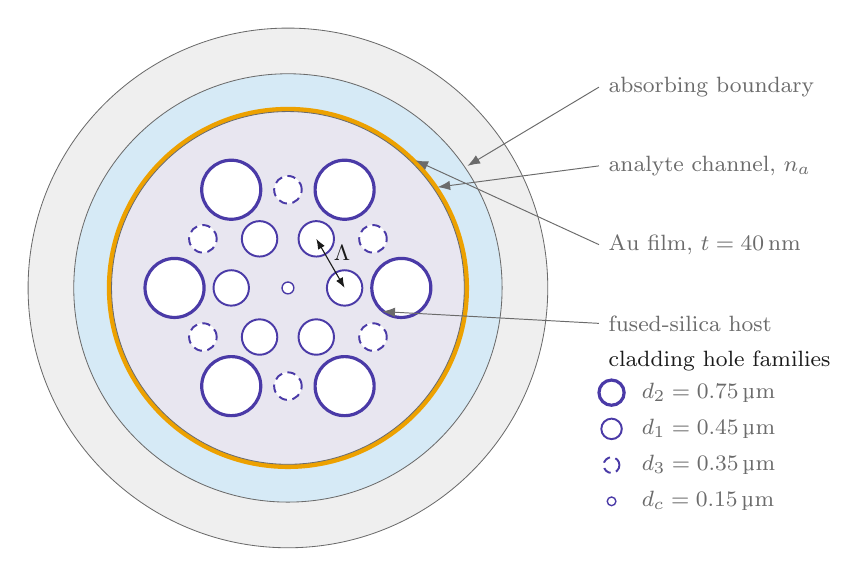
\begin{tikzpicture}[
    scale=1.0,
    every node/.style={font=\footnotesize},
    callout/.style={-{Latex[length=1.6mm]}, inkmuted, line width=0.35pt},
  ]

  % --- concentric regions, outermost first ---------------------------------
  \fill[pml, draw=inkmuted, line width=0.3pt] (0,0) circle (3.30);
  \fill[analyte, draw=inkmuted, line width=0.3pt] (0,0) circle (2.72);
  \fill[goldlayer] (0,0) circle (2.30);
  \fill[silica, draw=inkmuted, line width=0.3pt] (0,0) circle (2.24);

  % --- hexagonal cladding lattice -------------------------------------------
  % Pitch p in drawing units; three hole families keyed by radius and stroke.
  \def\p{0.72}

  % ring 1 (6 holes, radius r1) and ring 2 (12 holes, radius r2/r3 alternating)
  \foreach \k in {0,...,5}{
    \pgfmathsetmacro{\ang}{60*\k}
    \fill[white, draw=holeedge, line width=0.7pt]
      ({\p*cos(\ang)},{\p*sin(\ang)}) circle (0.225);
  }
  \foreach \k in {0,...,5}{
    \pgfmathsetmacro{\ang}{60*\k}
    \fill[white, draw=holeedge, line width=1.15pt]
      ({2*\p*cos(\ang)},{2*\p*sin(\ang)}) circle (0.375);
  }
  \foreach \k in {0,...,5}{
    \pgfmathsetmacro{\ang}{60*\k+30}
    \fill[white, draw=holeedge, line width=0.7pt, densely dashed]
      ({1.732*\p*cos(\ang)},{1.732*\p*sin(\ang)}) circle (0.175);
  }

  % central defect hole
  \fill[white, draw=holeedge, line width=0.5pt] (0,0) circle (0.075);

  % --- pitch vector between two adjacent first-ring centres -----------------
  \draw[{Latex[length=1.3mm]}-{Latex[length=1.3mm]}, ink, line width=0.4pt]
    ({\p*cos(0)},{\p*sin(0)}) -- ({\p*cos(60)},{\p*sin(60)});
  \node[ink, anchor=south west, inner sep=1pt]
    at ({0.5*\p*(cos(0)+cos(60))},{0.5*\p*(sin(0)+sin(60))}) {$\Lambda$};

  % --- region callouts ------------------------------------------------------
  \draw[callout] (3.95,2.55) -- (2.28,1.55);
  \node[inkmuted, anchor=west] at (3.95,2.55) {absorbing boundary};

  \draw[callout] (3.95,1.55) -- (1.90,1.28);
  \node[inkmuted, anchor=west] at (3.95,1.55) {analyte channel, $n_a$};

  \draw[callout] (3.95,0.55) -- (1.62,1.62);
  \node[inkmuted, anchor=west] at (3.95,0.55) {Au film, $t=40$\,nm};

  \draw[callout] (3.95,-0.45) -- (1.20,-0.30);
  \node[inkmuted, anchor=west] at (3.95,-0.45) {fused-silica host};

  % --- hole-family legend ---------------------------------------------------
  \begin{scope}[shift={(3.95,-1.55)}]
    \node[ink, anchor=west] at (0,0.62) {cladding hole families};
    \fill[white, draw=holeedge, line width=1.15pt] (0.16,0.22) circle (0.16);
    \node[inkmuted, anchor=west] at (0.42,0.22) {$d_2 = 0.75$\,\textmu m};
    \fill[white, draw=holeedge, line width=0.7pt] (0.16,-0.24) circle (0.13);
    \node[inkmuted, anchor=west] at (0.42,-0.24) {$d_1 = 0.45$\,\textmu m};
    \fill[white, draw=holeedge, line width=0.7pt, densely dashed]
      (0.16,-0.70) circle (0.10);
    \node[inkmuted, anchor=west] at (0.42,-0.70) {$d_3 = 0.35$\,\textmu m};
    \fill[white, draw=holeedge, line width=0.5pt] (0.16,-1.16) circle (0.055);
    \node[inkmuted, anchor=west] at (0.42,-1.16) {$d_c = 0.15$\,\textmu m};
  \end{scope}

\end{tikzpicture}
\end{document}
